\section{Low level taggers}

There are two types of low-level algorithms that are employed by the 

While the IP-based algorithms take input a set of tracks and just use the individual track features (such as IPs) to classify the jet, the vertexing-based algorithms (SV1 and JF) involve an iterative approach to reconstruct the topology of the displayed decay.


The outlining of this section is as follows: I first 

Although the RNNIP algorithm was proposed before developing my thesis, a key contribution of my thesis work was continuing to optimize this develop

\subsection{IP2D and IP3D}

\subsubsection{Lifetime signage}

\begin{figure}[htbp]
  \centering
 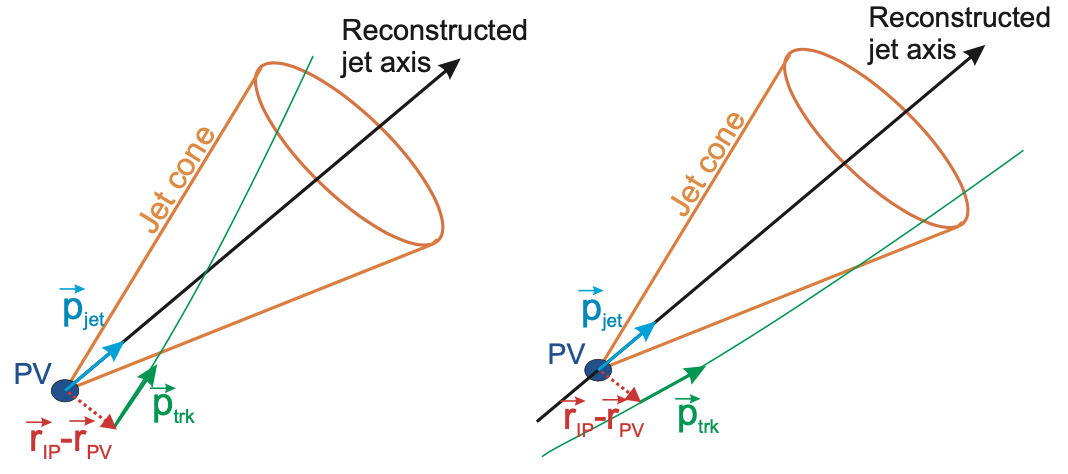
\includegraphics[width=0.5\textwidth]{figures/ftag/lifetime-signage}
 \caption{Lifetime signage graphic (from \cite{giacinto-thesis})}
 \label{fig:lifetime-signage}
\end{figure}


\textbf{3d sign}


$\Delta \vec{r}_{IP} = \vec{r}_{IP}  - \vec{r}_{PV} $

\begin{equation}
  \text{sign}_{3D} =   \text{sign} \left( \left[ \vec{p}_{trk} \times \vec{p}_{jet} \right] \cdot \left[   \vec{p}_{trk} \times \Delta \vec{r}_{IP} \right] \right)
  %\label{eq:}
\end{equation}

\textbf{2d sign}

\begin{equation}
  \text{sign}_{r \phi} =   \text{sign} \left( \sin \left( \phi_{jet} - \phi_{trk} \right) \cdot d_{0,trk} \right)
  %\label{eq:}
\end{equation}

\begin{equation}
  \text{sign}_{z} =   \text{sign} \left(  \left(  \eta_{jet} - \eta_{trk} \right) \cdot z_{0,trk}  \right)
  %\label{eq:}
\end{equation}



(Equations taken from Giacinto's thesis  \cite{giacinto-thesis}.)

\textbf{How are the IPs signed for the IP2D and IP3D algorithms}

\begin{itemize}
	\item \textbf{IP2D: }
	\begin{itemize}
	\item$d_0$ signed based on the projection of the vectors in the (x,y) plane
	\end{itemize}

	\item \textbf{IP3D:}
	\begin{itemize}
	\item $d_0$ signed with the 3D vectors
	\item $z_0$ signed based on the $(r, \phi)$ plane
\end{itemize}
\end{itemize}

\subsubsection{Mathematical motivation}


\begin{figure}[htbp]
  \centering
 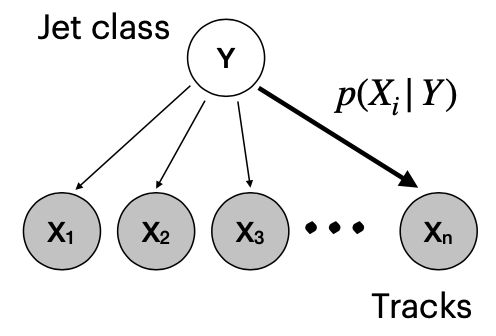
\includegraphics[width=0.5\textwidth]{figures/ftag/Naive-Bayes-illustration}
 \caption{Probabilistic graphical model illustration for a Naive Bayes algorithm.  }
  \label{fig:Naive-Bayes-illustration}
\end{figure}

%%%%%%%%%%%%%%%%%%%%%%%%%%%%
% Plot showing the non-independence of the tracking inputs
%%%%%%%%%%%%%%%%%%%%%%%%%%%%

%\def\figpath{figures/ftag/ATL-PHYS-PUB-2017-003/}
\begin{figure}[htbp]
  \centering
  \subfloat[]{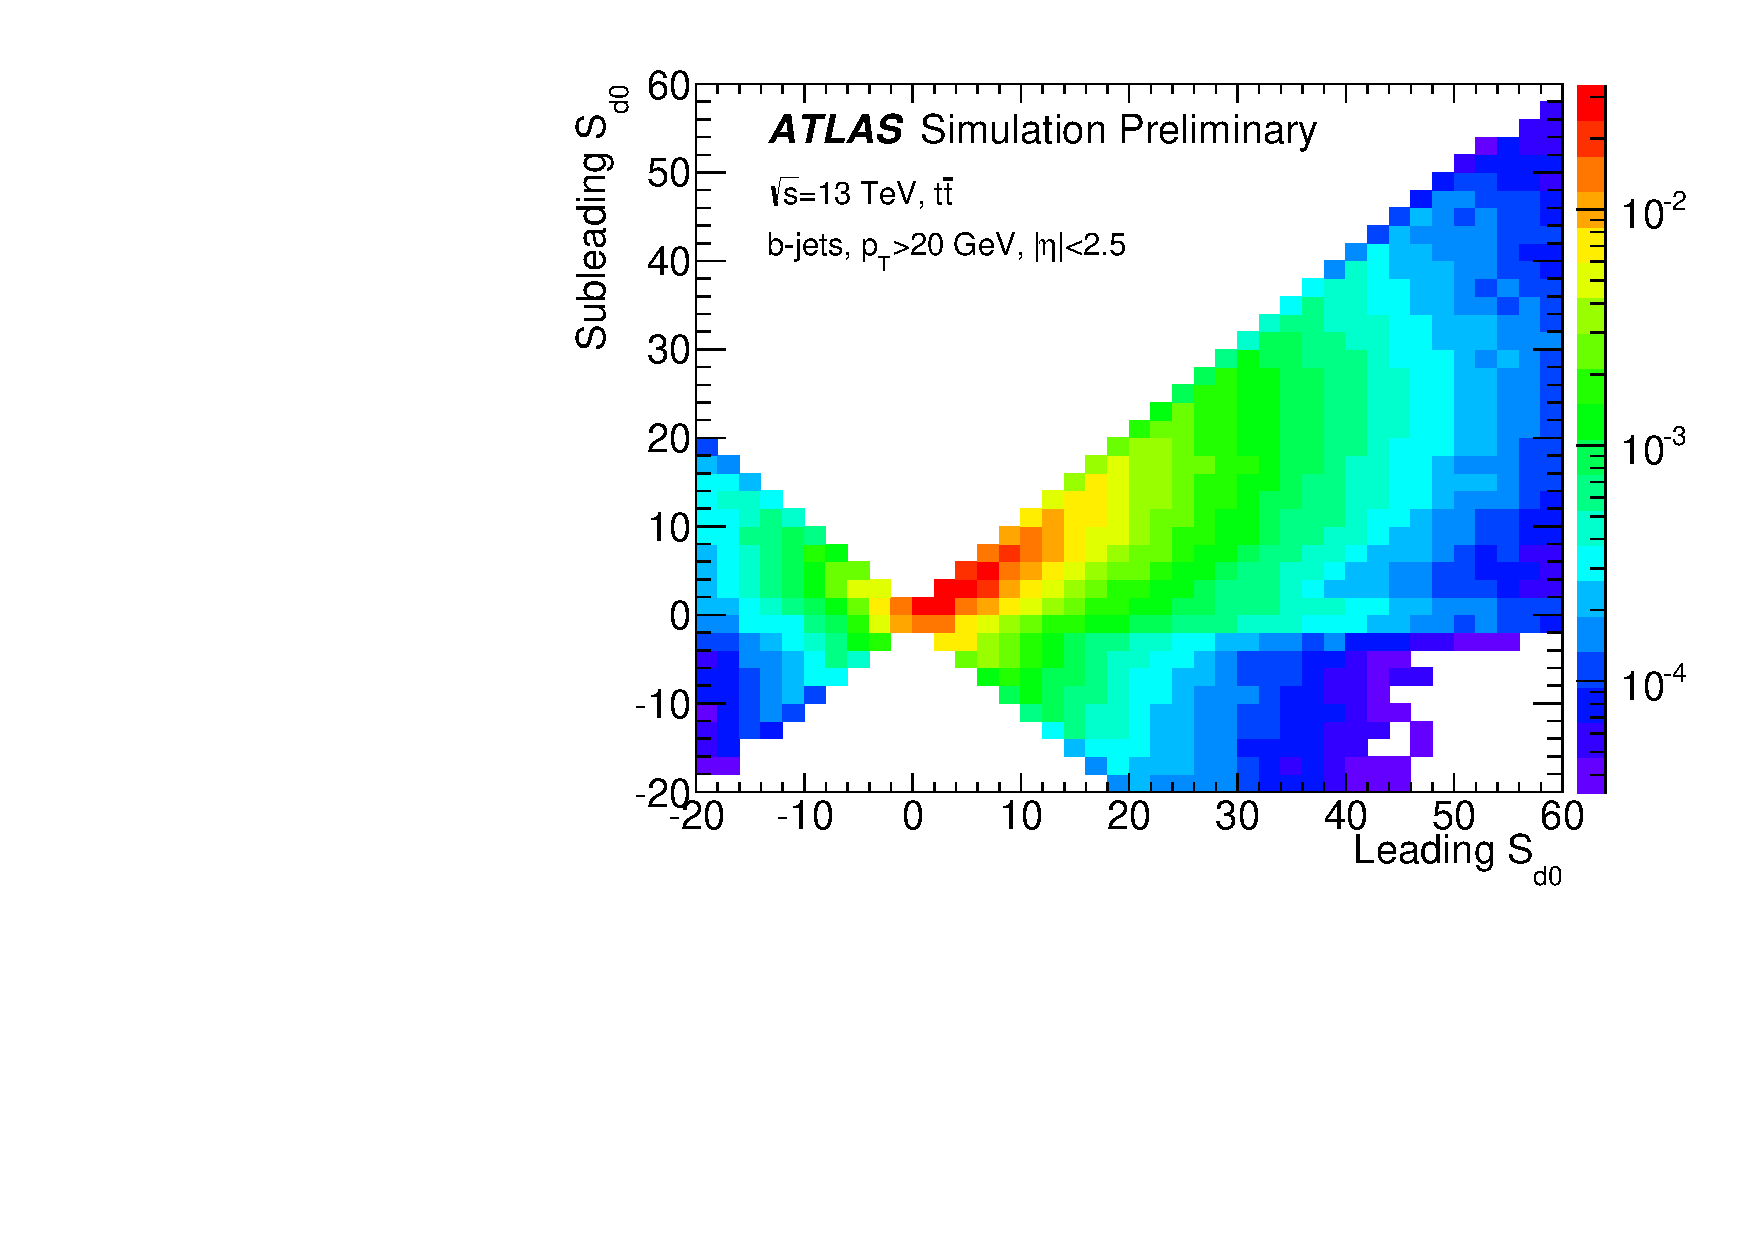
\includegraphics[width=0.5\textwidth]{figures/ftag/ATL-PHYS-PUB-2017-003/fig_01a}}
  \subfloat[]{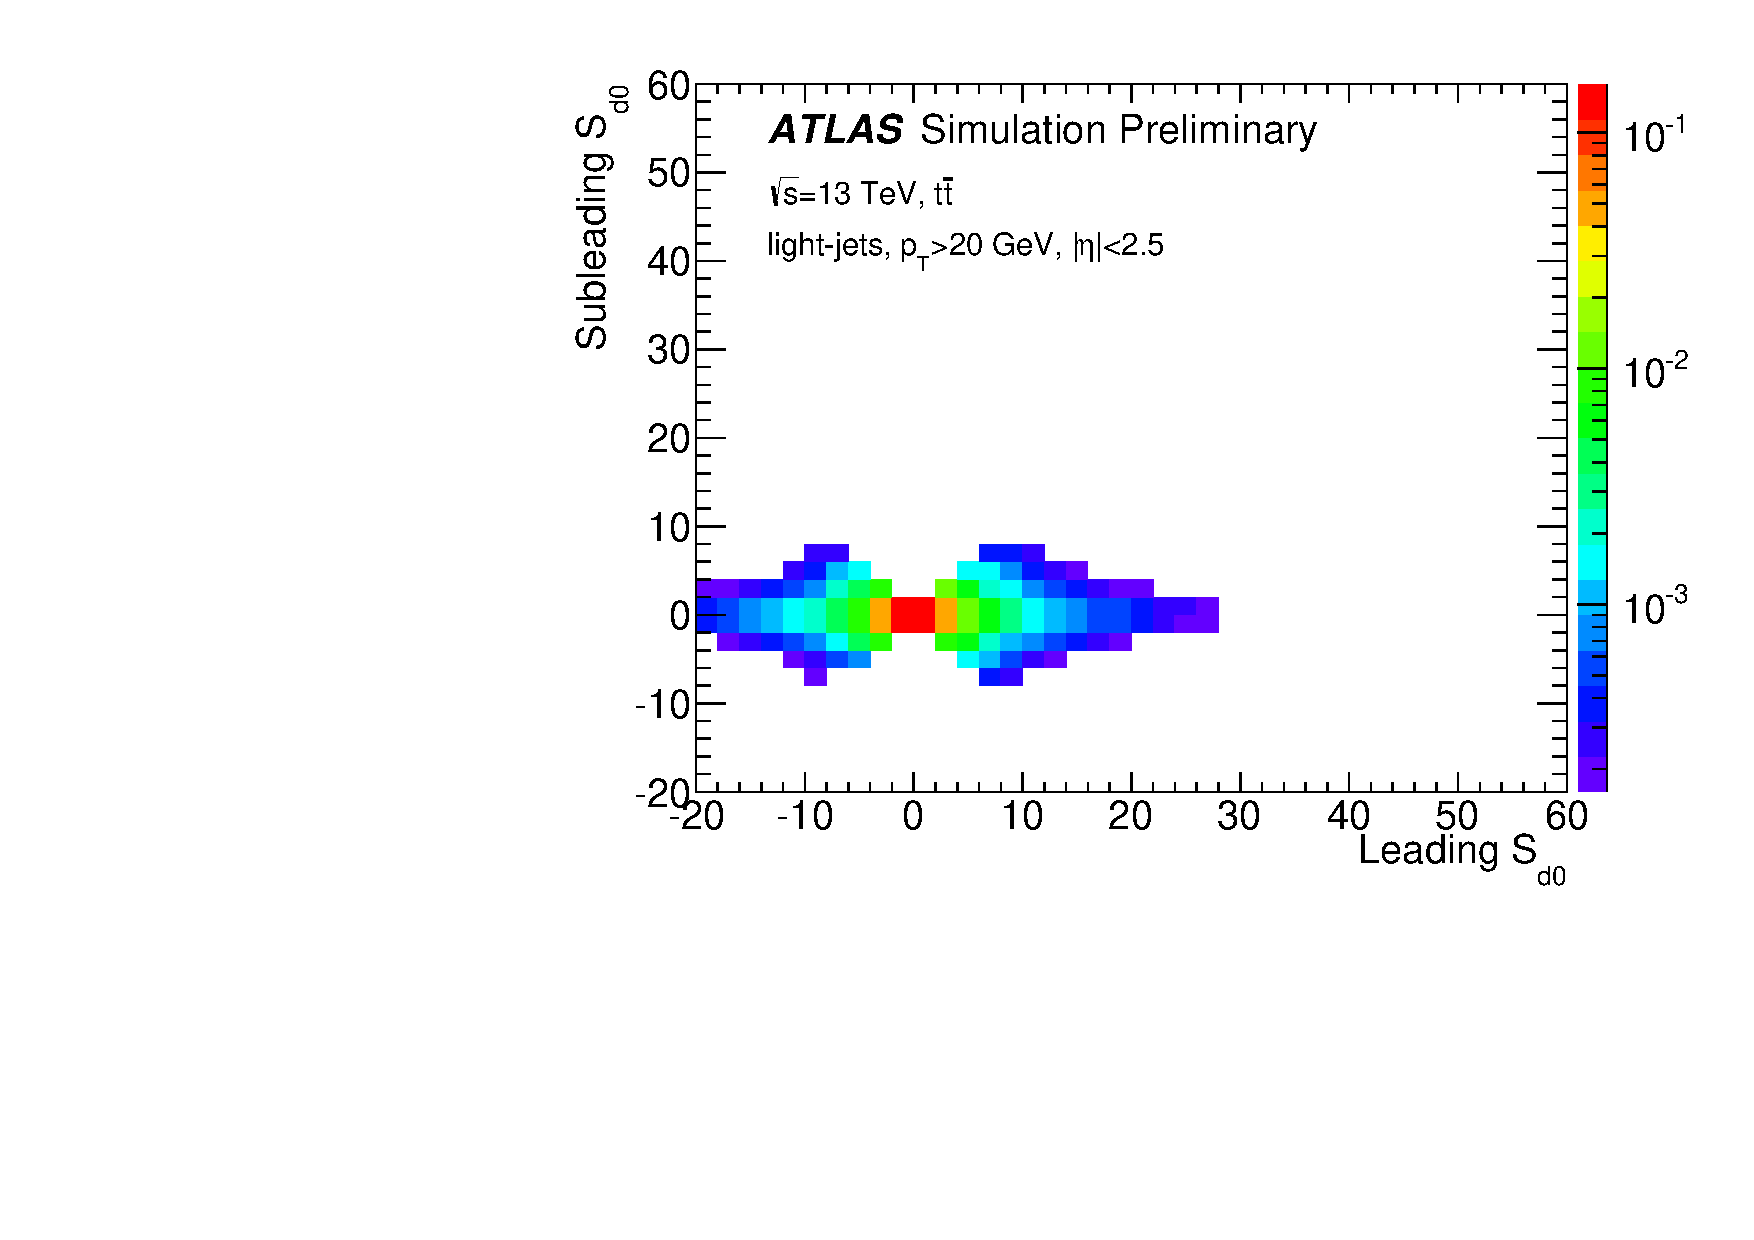
\includegraphics[width=0.5\textwidth]{figures/ftag/ATL-PHYS-PUB-2017-003/fig_01b}}
  \caption{ \cite{ATL-PHYS-PUB-2017-003}}
  \label{fig:rnnip-note-trk-ind}
\end{figure}


\subsubsection{Algorithm description}

% I don't think I need to describe the benefit of IP based algorithms
%\textbf{Should I mention that the lifetime signage is different between IP2D and IP3D? No - beyond the scope!}


The IP3D algorithm \cite{FTAG-2018-01} assigns probabilities to tracks based on two-dimensional likelihood templates, with the tracks' $z_0\sin\theta$ and $d_0$ lifetime signed significances, built from simulated jets.
These templates are obtained in 14 exclusive categories defined by the hit patterns of the tracks, and separately for tracks in $b$-jets, $c$-jets and light-flavour jets. 
The inclusive distribution of $z_0\sin\theta$ and $d_0$ lifetime signed significances for the different jet flavours are shown in Figure \ref{fig:flippedInputs}.
% The IP3D algorithm builds histograms for estimating the likelihood distribution of the IP significance for the tracks in $b$-jets and $l$-jets in 14 exclusive categories defined by the hit patterns of the tracks \cite{FTAG-2018-01}. 
By assuming that the track probabilities inside a jet are independent, jet-level likelihoods can be constructed by multiplying the individual probabilities.
The IP3D $b$-tagging discriminants are therefore defined as:
\begin{equation}
D_{\text{IP3D,l}} = \log \prod_{i \in \text{tracks}} \frac{p_b^i}{p_l^{i}} \qquad D_{\text{IP3D,c}} = \log \prod_{i \in \text{tracks}} \frac{p_b^i}{p_c^{i}}.
\end{equation}
% multiplication over the track likelihoods produces a jet level probability, and the ratio of jet probabilities from the $l$ and $b$ hypotheses defines the $b$-tagging discriminant: $\log \prod_{i \in tracks} p_b^{(i)} / p_l^{(i)}$.
RNN based IP algorithms aim to overcome this overly simplistic assumption of independence, and offer the possibility to employ more features than only the IP significance in the discriminant~\cite{ATL-PHYS-PUB-2017-003}. 

%%%%%%%%%%%%%%%%%%%%%%%%%%%%
% Plot from the DIPS note
%%%%%%%%%%%%%%%%%%%%%%%%%%%%
\def\figpath{figures/ftag/dips-note/}
\begin{figure}[htbp]
  \centering
  \subfloat[]{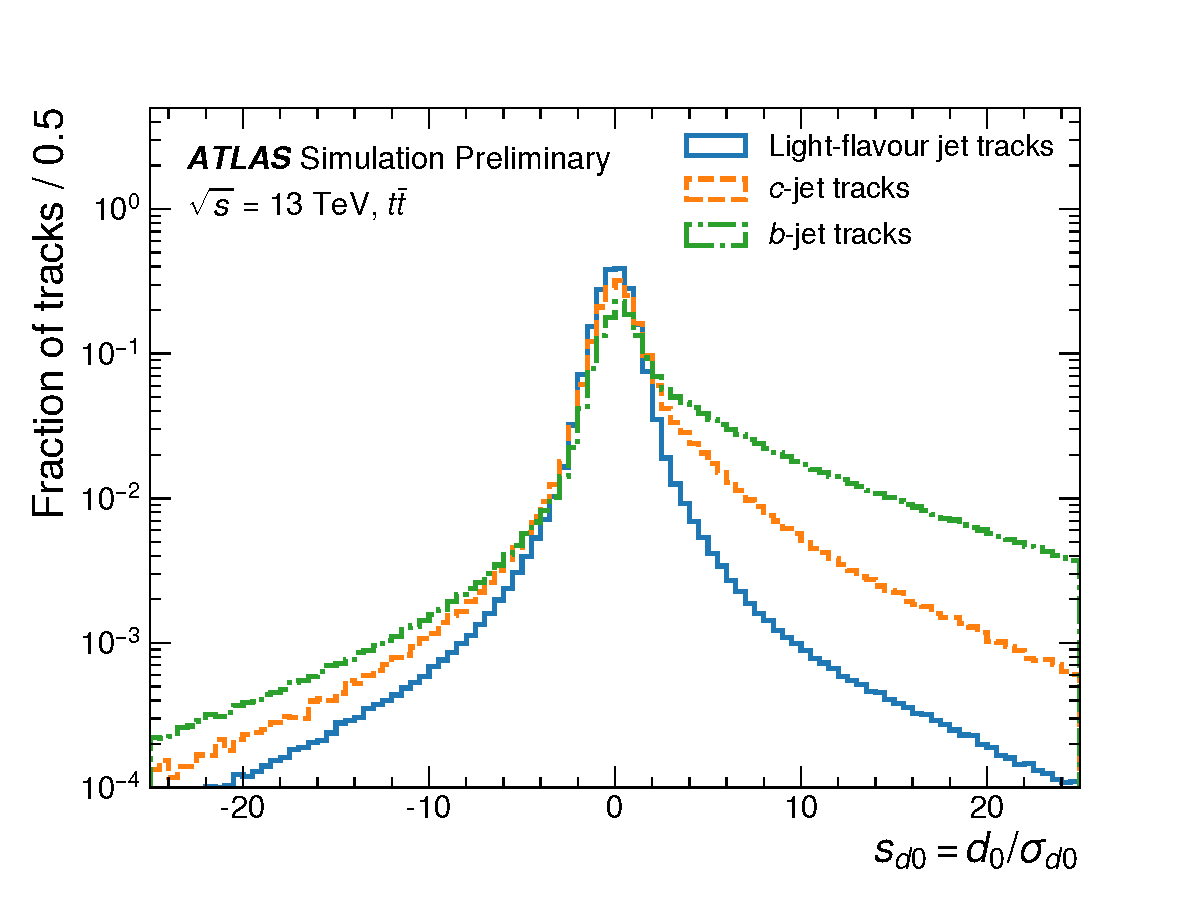
\includegraphics[width=0.5\textwidth]{\figpath/sd0}}
  \subfloat[]{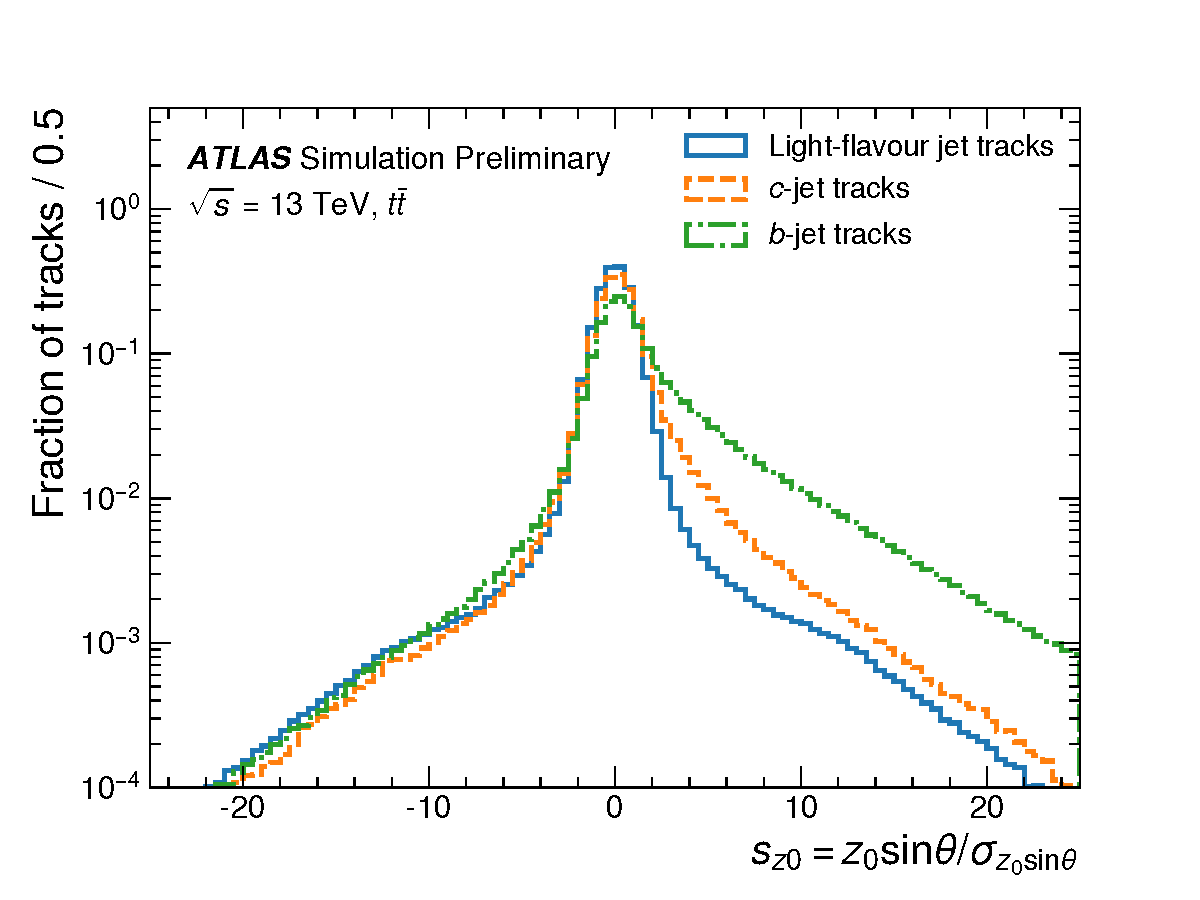
\includegraphics[width=0.5\textwidth]{\figpath/sz0}}
  \caption{Lifetime signed transverse (a) and longitudinal (b) significances for $b$-jets, $c$-jets and light-flavor jets.}
  \label{fig:flippedInputs}
\end{figure}





%%%%%%%%%%%%%%%%%%%%%%%%%%%%%%%%
% Table of the IPXD categories
%%%%%%%%%%%%%%%%%%%%%%%%%%%%%%%%

\begin{table}[h!]
  \begin{center}
    \begin{adjustbox}{width=\columnwidth,center}
    \begin{tabular}{ l | l | c c c  } % <-- Alignments: 1st 2 cols left, last three 3rd right, with vertical lines in between
      {} & {} &  \multicolumn{3}{ c }{ Fractional contribution [\%] } \\
      \textbf{\#} & \textbf{Category}  & \Pqb-jets & \Pqc-jets & light-jets  \\
      \midrule 
      0 & No hits in first two layers; expected hit in IBL and b-layer & 1.9 & 2.0 & 1.9   \\
      1 & No hits in first two layers; expected hit in IBL and no expected hit in b-layer & 0.1 & 0.1 & 0.1 \\
      2 & No hits in first two layers; no expected hit in IBL and expected hit in b-layer & 0.04 & 0.04 & 0.04 \\
      3 & No hits in first two layers; no expected hit in IBL and b-layer & 0.03 & 0.03 & 0.03 \\
      4 & No hit in IBL; expected hit in IBL & 2.4 & 2.3 & 2.1 \\
      5 & No hit in IBL; no expected hit in IBL & 1.0 & 1.0 & 0.9  \\
      6 & No hit in b-layer; expected hit in b-layer & 0.5 & 0.5 & 0.5 \\
      7 & No hit in b-layer; no expected hit in b-layer & 2.4 & 2.4 & 2.2  \\
      8 & \emph{Shared} hit in both IBL and b-layer & 0.01 & 0.01 & 0.03  \\
      9 & At least one \emph{shared} pixel hits & 2.0 & 1.7 & 1.5  \\
      10 & Two or more \emph{shared} SCT hits & 3.2 & 3.0 & 2.7  \\
      11 & \emph{Split} hits in both IBL and b-layer & 1.0 & 0.87 & 0.6  \\ 
      12 & \emph{Split} pixel hit & 1.8 & 1.4 & 0.9 \\
      13 & Good quality & 83.6 & 84.8 & 86.4 
    \end{tabular}
    \end{adjustbox}
    \caption{Categories for defining the IP2D and IP3D templates \cite{ATL-PHYS-PUB-2017-013}.}
    \label{table:IPXD-categories}
  \end{center}
\end{table}


\subsubection{RNNIP}

\def\figpath{figures/ftag/dips-note/}

Tracks are reconstructed from energy deposits, or hits, in the inner detector system and are required to pass a quality selection: 
each track must have at least 7 hits in the silicon layers (pixel and SCT, where dead sensors are not penalized), 
no more than two missing hits where expected in the silicon layers, 
no more than one hit shared by multiple tracks, 
at least one hit in the pixel detector, and $|\eta| < 2.5$. 

%\subsection{Algorithm overview}

% from dips intro
% The choice of the RNN architecture was motivated by the capability to operate over jets with variable numbers of tracks, while the use of neural networks provided the flexibility to add more information about the track kinematics into the tagging discriminant.
%while avoiding the "curse of dimensionality" inherit when using histograms to build up likelihood templates \cite{papamakarios2019neural}.
%By modelling the jet as a sequence (or an ordered set of tracks) the RNN can operate over an arbitrary number of associated 


RNNs operate on variable length \emph{sequences} by iterating over the sequence elements, processing them with a neural network, and using previously processed elements when processing new ones. 
It then outputs a fixed size vector that can be used for classification. 
The RNNIP algorithm utilizes a Long Short Term Memory (LSTM) cell for the RNN to preserve long range correlations between the elements of the sequence \cite{LSTMs}. 
As shown in \cite{ATL-PHYS-PUB-2017-003}, the accounting for these correlations allows the RNN to be more performant than IP3D even when trained on the same inputs.
The use of neural networks instead of histograms allows one to avoid the "curse of dimensionality" when using additional variables sensitive to the kinematics of the $b$-hadron decay which significantly improve performance \cite{ATL-PHYS-PUB-2017-003}.
%The benefit of using an RNN as opposed to a standard multi-layer perceptron is that the RNN architecture that can operate natively over varying length inputs (i.e, a varying number of tracks in the jet) by sharing weights for the operations that update the hidden states. This allows the RNN to train with fewer parameters to get a similarly performing network \cite{need ref}.


\begin{figure}[htbp]
\centering
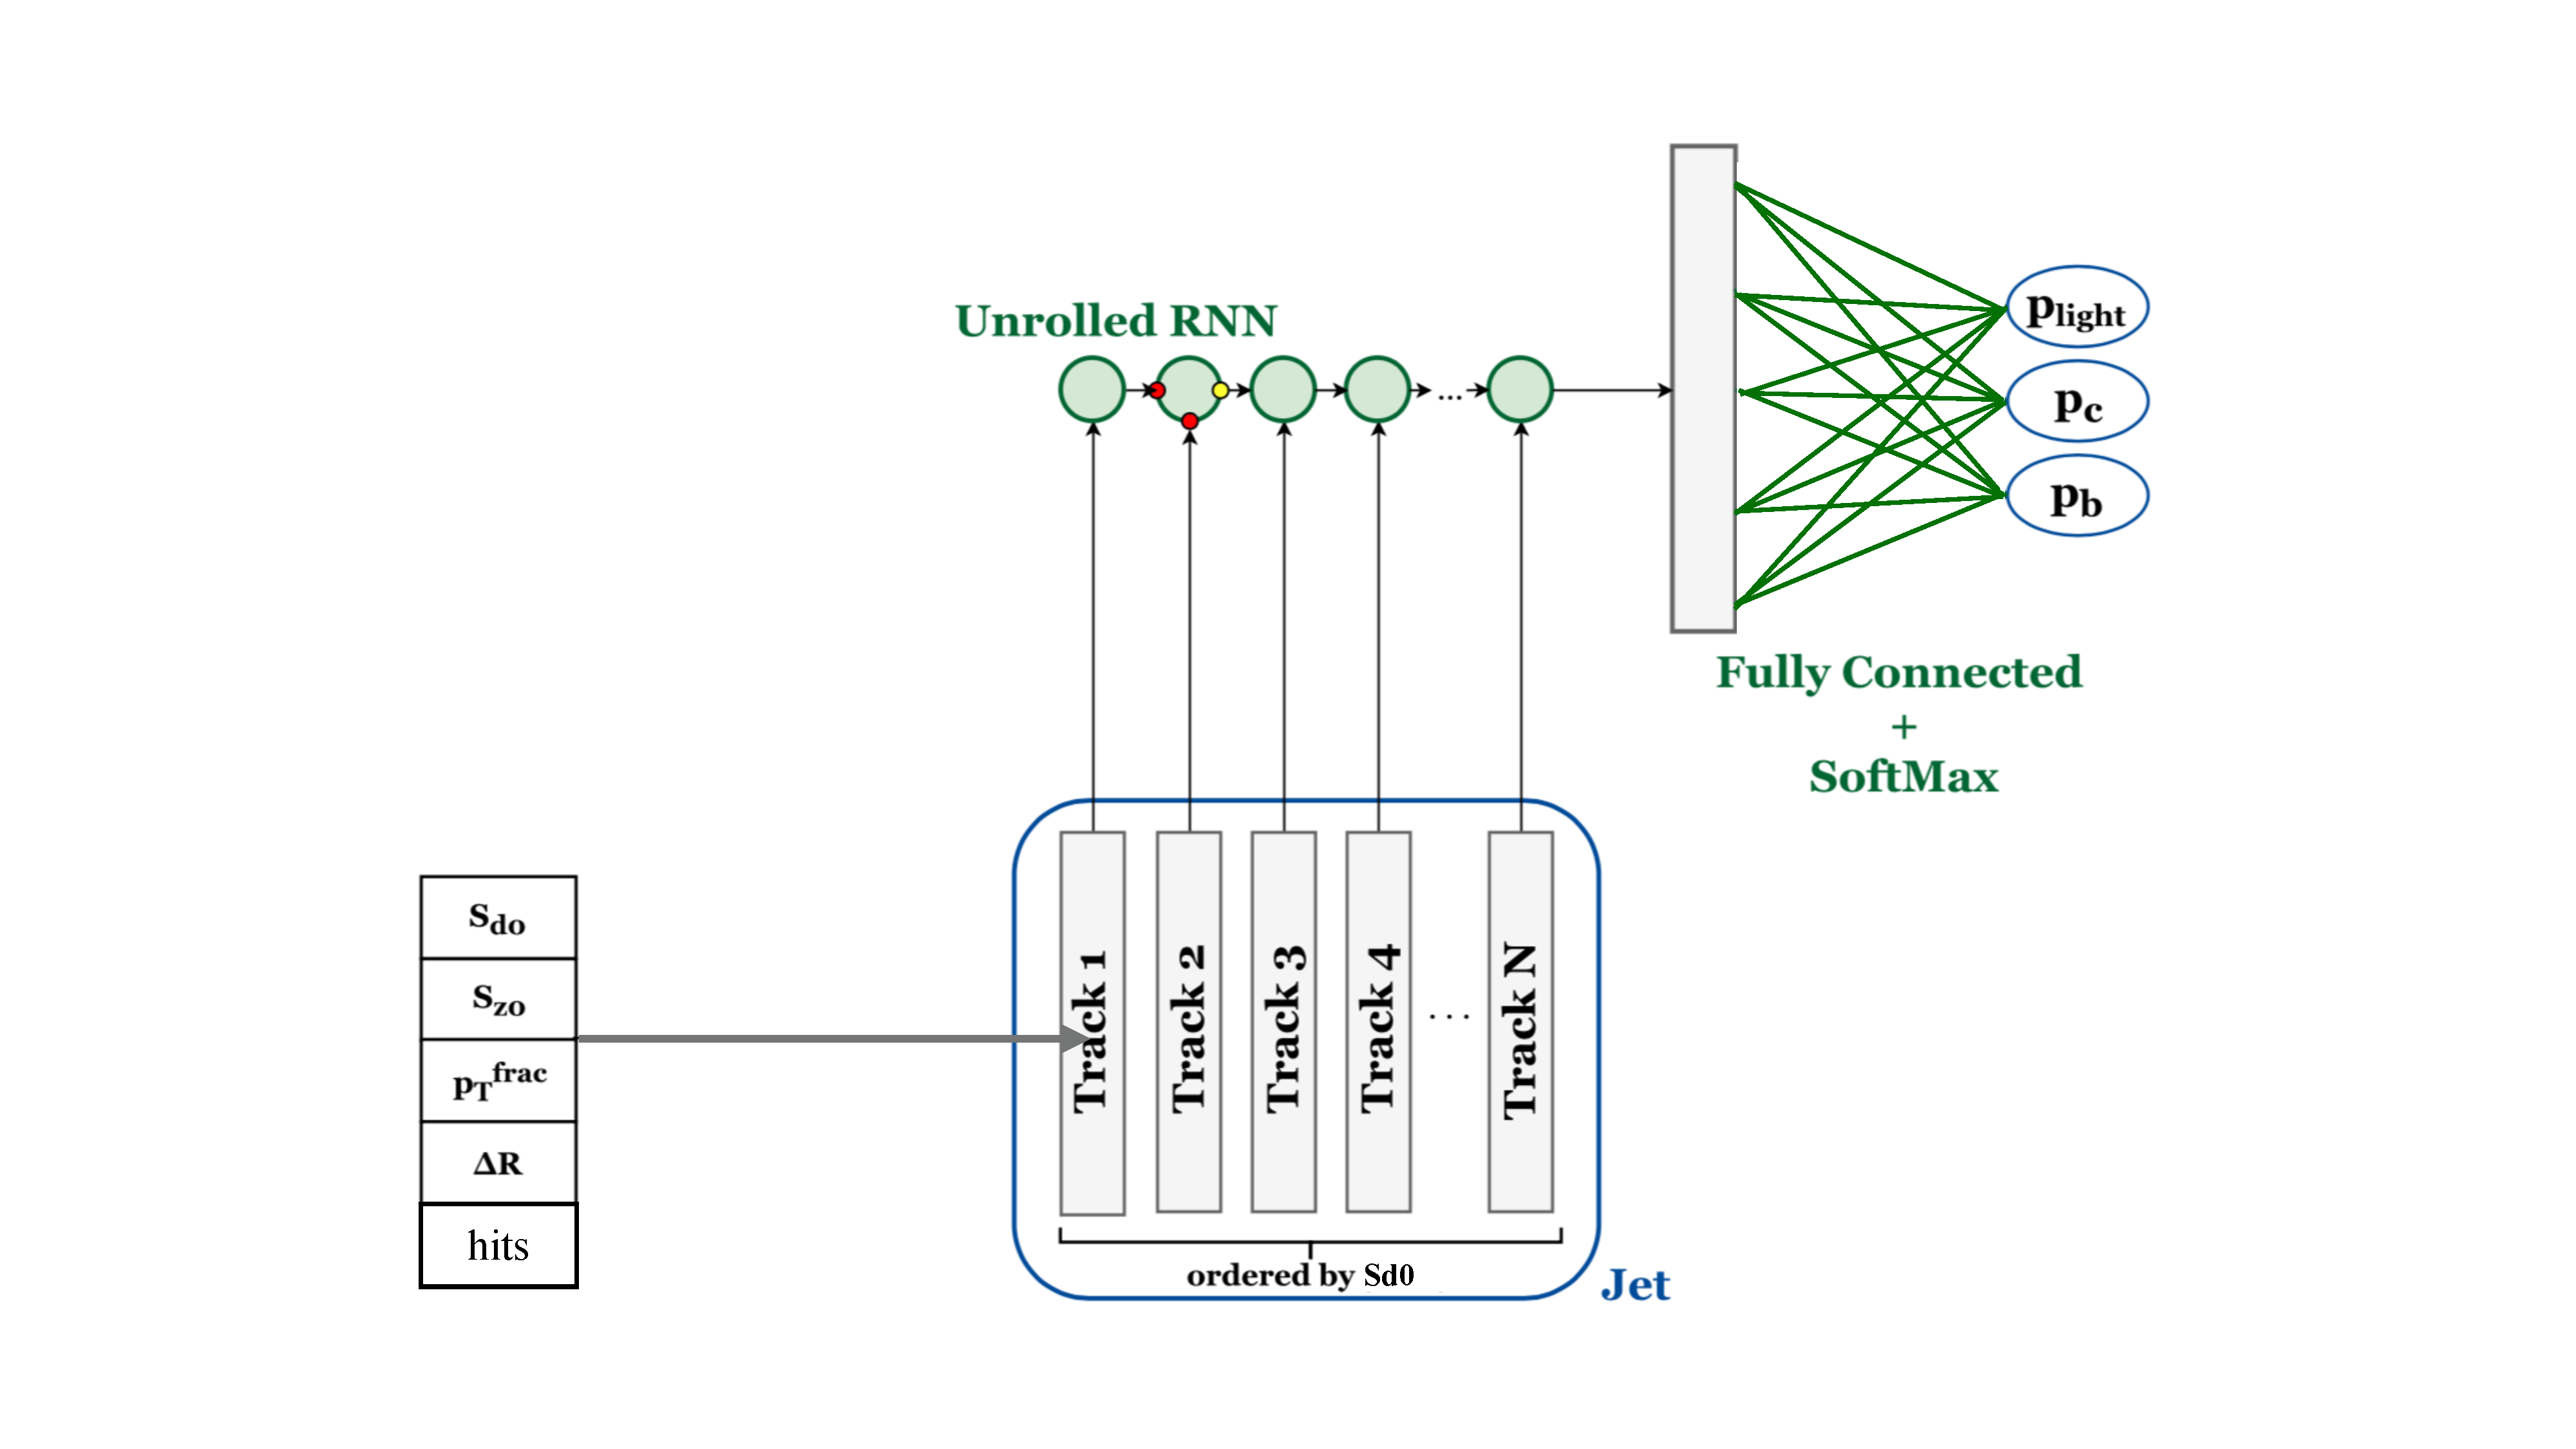
\includegraphics[width=0.8\linewidth]{figures/ftag/RNN-graphic}
\caption{RNNIP architecture (modified from \ref{ATL-PHYS-PUB-2017-003}).}
 \label{fig:RNN-graphic}
\end{figure}


An implementation of the RNNIP algorithm is used as the baseline for comparison to DIPS, but has further optimisations with respect to~\cite{ATL-PHYS-PUB-2017-003}. The RNNIP architecture comprises a 100 dimensional LSTM hidden state and a dropout layer, with dropout fraction of 0.2, before a 20 unit fully connected layer for classification, uses track IP significance, kinematics, and the number of hits in the silicon detectors as features (described in Table~\ref{table:inputs}), and orders the tracks by $s_{d_0}$.
%The RNNIP presented here has some modifications with respect to the one in \cite{ATL-PHYS-PUB-2017-003}. First, since the original RNNIP presentation, significant work has gone into the calibration of the high level tagger, DL1r, which includes as inputs the RNNIP outputs. The measurement of the data-to-MC scale factors in $l$-jets poses a unique challenge since even if we start with a l-jet dominated sample, our $b$-taggers are so powerful that cutting on the $b$-tagging discriminant gives a $b$-jet dominated sample that makes it infeasible to measure the $l$-jet efficiency directly in data. To account for this, we instead design a "flipped" tagger such that the performance on $l$-jets stays the same, but the performance on identifying $b$-jets is dramatically reduced \cite{ATLAS-CONF-2018-006}. Since the large impact parameters for $l$-jets are dominantly from resolution effects, they are mostly symmetric about 0, while the HF tracks from the long lived hadron decay bias the IP distributions in $b$-jets to positive values, as shown in Figure~\ref{fig:flippedInputs}. Therefore, the flipped versions of the RNNIP and IPXD taggers just change the sign of the IP inputs to reduce the $b$-tagging efficiency. The RNNIP presented in \cite{ATL-PHYS-PUB-2017-003} ordered the tracks by an $|s_{d0}|$ sort, but this washes away\footnote{Too informal - when I have data look up ananyms for ameliorate} some of the information we were trying to encode for the flipped tagger. The RNN presented here and in the more recent \cite{PFlowPublicPlots2019} the tracks were therefore ordered by $s_{d0}$ instead. In addition, previously, to be compatible with RNNIP the same inputs were used as the IPXD algorithms by taking the category encoding the track quality in an 2-dimensional embedding before feeding it in as an input to the LSTM. Now we simply feed in the hits variables which went into the IPXD category definitions, which led to an $\mathcal{O}\left(10\%\right)$ improvement for the $l$ rejection at a the 60\% efficiency for identifying $b$-jets.\footnote{Rejection hasn't been defined yet in the note - should I take this number out?} Finally the architecture has been modified. The size of the LSTM hidden state has been increased to 100 for $t\bar{t}$ trainings and 400 for the extended hybrid sample, where the size of the hidden state was optimised for each physics sample. Additionally, in the final layer before classification, a dropout layer has been added with a dropout fraction of 0.2 to improve the network's generalization to the test set \cite{Dropout}, and then the hidden state is fed through a fully connected layer with 20 hidden units before the softmax layer.

%\subsection{Optimizations}


\begin{table}[h!]
  \centering
    \begin{tabular}{l | l } % <-- Alignments: 1st column left, 2nd middle and 3rd right, with vertical lines in between
      \textbf{Input} & \textbf{Description}  \\
      \hline
      \hline
  $s_{d0}$ & $d_0 / \sigma_{d0}$: Transverse IP significance \\
	$s_{z0}$ & $z_0 \sin \theta / \sigma_{z0 \sin \theta}$: Longitudinal IP significance \\
	$\log \pT^{frac}$ & $\log \pT^{track} / \pT^{jet}$: Logarithm of fraction of the jet $\pT$ carried by the track \\
	$\log \Delta R$ & Logarithm of opening angle between the track and the jet axis \\
	IBL hits & Number of hits in the IBL: could be \{ 0, 1, or 2 \} \\
	PIX1 hits & Number of hits in the next-to-innermost pixel layer: could be \{ 0, 1, or 2 \} \\
	shared IBL hits & Number of shared hits in the IBL \\
	split IBL hits & Number of split hits in the IBL \\
	nPixHits & Combined number of  hits in the pixel layers \\
	shared pixel hits & Number of shared hits in the pixel layers \\
	split pixel hits &  Number of split hits in the pixel layers \\
	nSCTHits  & Combined number of hits in the SCT layers \\
	shared SCT hits & Number of shared hits in the SCT layers \\
    \end{tabular}
    \caption{Track features used as inputs for RNNIP and DIPS algorithms.}
    \label{table:inputs}
\end{table}



\subsection{SV1}
\label{subsec:sv1}

\def\figpath{figures/ftag/ANA-FTAG-2019-07-PAPER/sv1}

\textbf{Philosophy:} 

SV1 is a vertexing algorithm that reconstructs displaced decays where the set of tracks come from a single secodary vertex.
Although strictly speakig this will rarely be 

Set of input tracks (preselection):
\begin{itemize}
	\item Track cuts: $|d_0| < 3.5\mathrm{mm}$, $|z_0 \sin \theta| < 5\mathrm{mm}$ \cite{giacinto-thesis} and $\pt > 500$~MeVs.
	\item Some track cleaning cuts for jets with $\eta > 1.5$ (since these tracks pass through more material).
	\item Also - only take the 25 highest \pt tracks inside of the jet (helped for reducing the reconstruction of vertices from a random crossing of tracks at high jet \pt \cite[ATL-PHYS-PUB-2017-011].   
\end{itemize}

These track pre-selection cuts are looser than the IPXD (and RNNIP) algorithms because the next step of selecting the tracks originating from the same point in space acts as another cut on the input tracks. The track \ldots



\begin{itemize}
	\item Form all pairs of 2-track vertices satisfying \cite{giacinto-thesis}:
	\begin{enumerate}
		\item Prob$(\chi^2_{2-trk vtx}) > 3.5$\%
		\item Each track needs to be displaced from the PV with a significance $L_{3D} / \sigma(L_{3D}) > 2\sigma$ and the sum of the two-track significances larger than 6.\footnote{$L_{3D}$ is the 3d distance from the tracks POCA to the PV.}
		\item These tracks need to be ``downstream'' of the jet axis ($\left( \vec{r}_{2 trk} - \vec{r}_{primary} \right) \cdot \vec{p}_{jet} $) \hl{What is $\vec{r}_primary$?}
	\end{enumerate}
	\item Veto tracks that form 2-track vertices consistent with\footnote{The tracker only measures the momentum of the particle, so to reconstruct a mass, we need to make an assumption for what the particle ID is for the mass of the track to get the 4-vector. The meson (or lepton) mass used for each track to reconstruct the 2-track vertex invariant mass is denoted by the subscripts. \hl{I took these numbers from the JF pub note, will need to confirm is they are the same for SV1.}}:
	\begin{enumerate}
		\item $K_s$ decays ( $|m_{\pi^+ \pi^-} - m_{K^0}| < 18$~MeV )
		\item $\lambda$ decays ( $|m_{p \pi^-} - m_{K^0}| < 18$~MeV )
		\item $\gamma$ conversions ($m_{ee} < 30$~MeV)  
		\item hadronic material interactions (veto vertex interactions that overlap with detector material)
	\end{enumerate}
	\item Iterate over this ``cleaned'' set of tracks fitting a single SV  
	\begin{itemize}
		\item If this vertex fix has a $\mathrm{Prob}(\chi^2_{vtx}) < 0.1\%$ -- or -- a vertex mass larger than 6~GeV, remove the track with the largest $\chi^2$ contribution and rise and repeat the fit.
	\end{itemize}	
\end{itemize}


For a true displaced decay, this secondary vertex will have properties consistent with a $B$ or $D$ hadron decay, and some key discriminating variables include the mass of the secondary vertex, the energy fraction, \hl{\ldots}

 \begin{figure}[htbp]
        \centering
        \subfloat[]{ 
                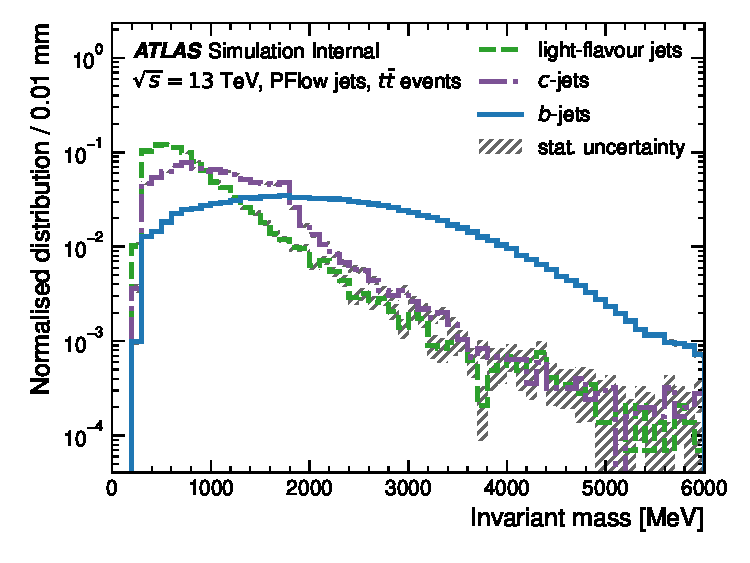
\includegraphics[width=0.32\linewidth]{\figpath/SV1_masssvx_ttbar}
        } 
         \subfloat[]{ 
                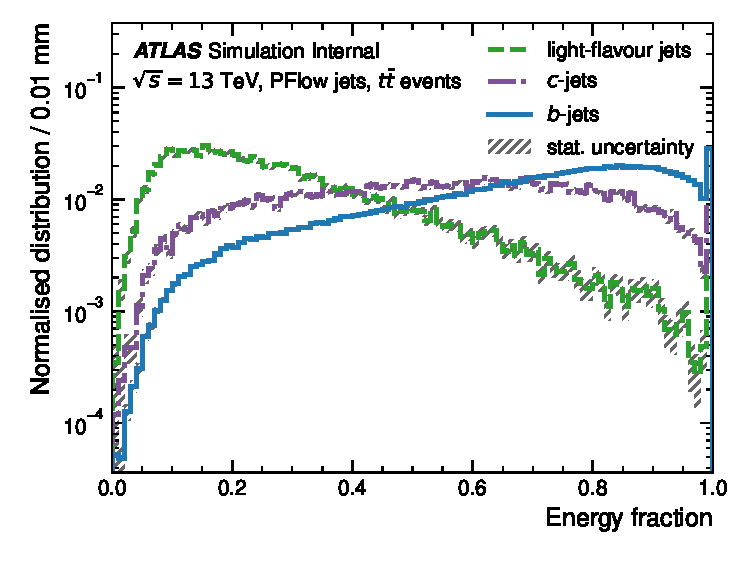
\includegraphics[width=0.32\linewidth]{\figpath/SV1_efracsvx_ttbar.pdf}
        } 
                 \subfloat[]{ 
                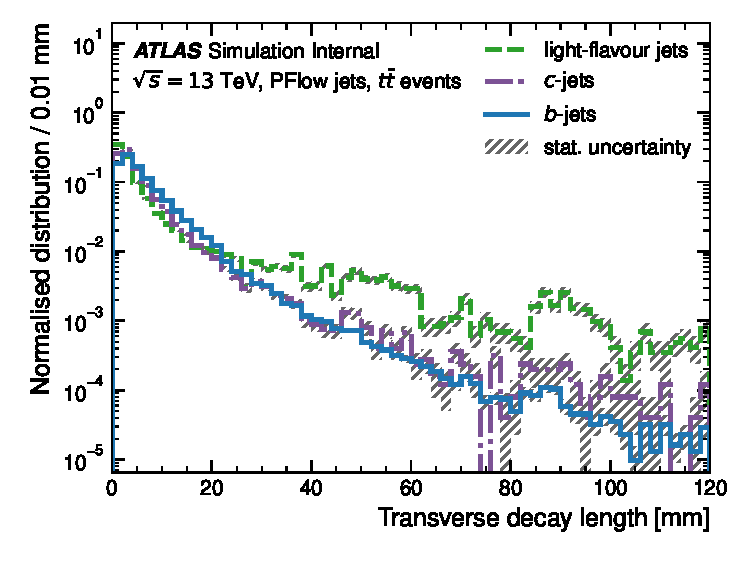
\includegraphics[width=0.32\linewidth]{\figpath/SV1_Lxy_ttbar.pdf}
        } \\ 
        \subfloat[]{ 
                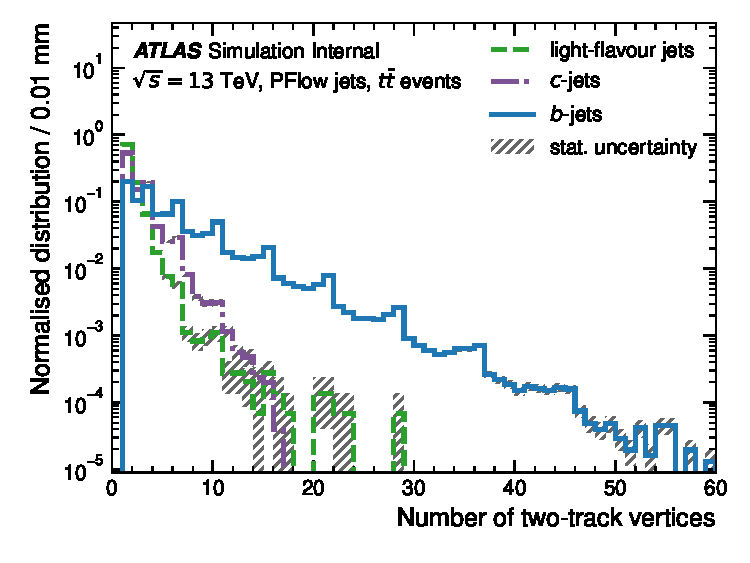
\includegraphics[width=0.32\linewidth]{\figpath/SV1_N2Tpair_ttbar.pdf}
        } 
         \subfloat[]{ 
                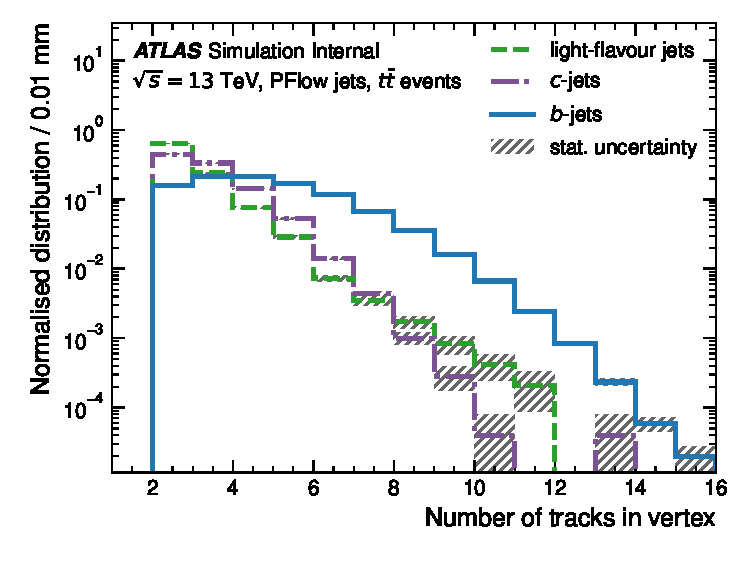
\includegraphics[width=0.32\linewidth]{\figpath/SV1_NGTinSvx_ttbar.pdf}
        } 
                 \subfloat[]{ 
                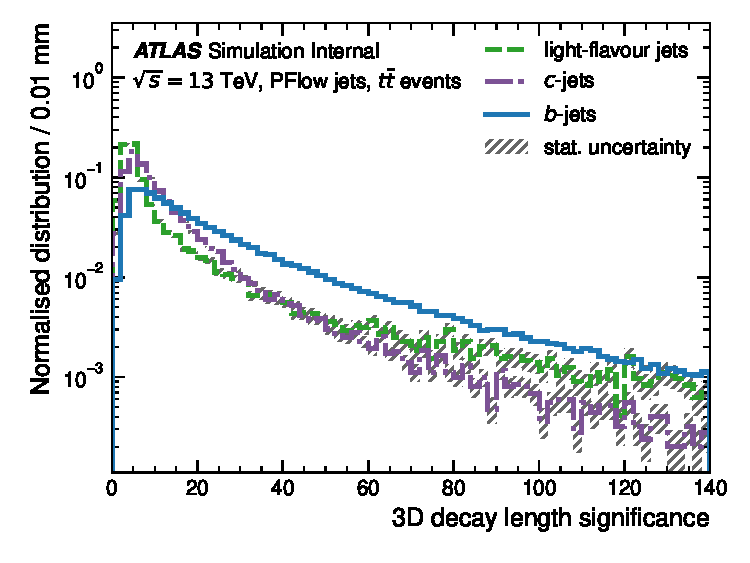
\includegraphics[width=0.32\linewidth]{\figpath/SV1_significance3d_ttbar.pdf}
        } 
        \caption{The SV1 inputs that (will be) in the FTAG algos paper \cite{ANA-FTAG-2019-07}.}
        \label{fig:sv1 inputs}
\end{figure}


\begin{table}[h!]
  \centering
    \begin{tabular}{p{4cm} | p{10cm}  }  
      \textbf{Input} & \textbf{Description}  \\
      \hline
      \hline
  	 $m$ & Invariant mass of the tracks reconstructed in the secondary vertex \\
	 $f_E$ &The energy of the SV over the energy of the jet \\
	 $\Delta R(\vec{p}_{jet},\vec{r}_{SV} - \vec{r}_{PV})$ & Opening angle between the jet and the SV flight axis \\
	 $L_{xy}$ & SV transverse distance from the PV \\
	 $L_{xyz}$ & SV distance from the PV \\
 	 $S_{xyz}$ & Significance of the displacement of the SV: $L_{xyz} / \sigma_{xyz}$ \\
	$n_{vtx \ trk}$ & Number of tracks in the SV \\
	$n_{2-trk vtx}$ & Number of 2 track vertices before the vertex fit \\
    \end{tabular}
    \caption{Features from the SV1 reconstruction that are fed as input to the DL1r tagger.}
    \label{tab:sv1-inputs}
\end{table}



\FloatBarrier
\clearpage
\subsection{JetFitter}
\label{subsec:jf}

\begin{itemize}
	\item Motivation for JF: Cascade topology
	\item Key assumption: Every (well motivated b/c the B-hadron carries a large portion of the initial quarks momentum which causes the B (and subsequent D) hadrons to form a line with respect to the
	\item Briefly sketch the extension to the KF formalism
	\item The track selection and JF algorithm
\end{itemize}

\begin{figure}
\centering
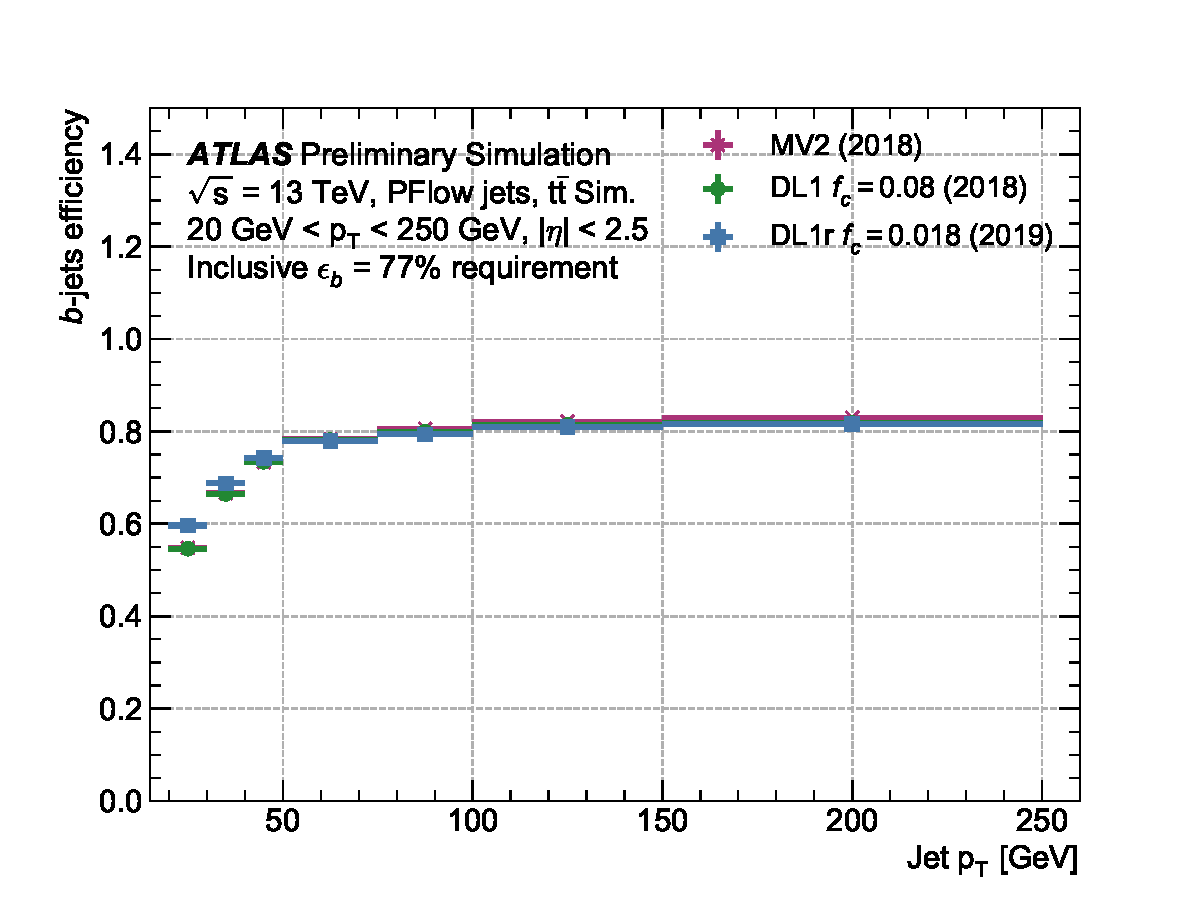
\includegraphics[width=.6\textwidth]{{figures/ftag/ATL-PHYS-PUB-2018-025/fig_02a.pdf}} 
% Note fig (b) shows the reconstruction level picture
\caption{\cite{ATL-PHYS-PUB-2018-025}}
\label{fig:jf-fig-02a}
\end{figure}

The tracks fed in as input to the JF algorithm have a loose selection criteria of $|d_0| < 3.5$~mm and $|z_0 \sin \theta| < 1.5$~mm, and $p_\text{T}^{trk} > 500~$MeV. 
The Kalman Filter formalism is extended to fit a number of secondary vertices, with the extended state vector (of the Hidden Markov Model) given by \Eq{\ref{eq:jf-state}}.
The key assumption of this algorithm is that all of the displaced vertices lie on the \emph{same} flight axis, characterized by the $(\phi,\theta)$ direction.
Then the cascade of $N$ displaced vertices are identified by the distance along this flight path from the PV (denoted by the $d_1, d_2, \ldots d_N$ distances).

\begin{equation}
\vec{d} = \left( x_{PV}, y_{PV}, z_{PV}, \phi, \theta, d_1, d_2, \ldots, d_N \right)
\label{eq:jf-state}
\end{equation}

The jet axis is used to initialize $(\phi,\theta)$, and the N displaced vertices are considered for the tracks intersecting this flight axis. % p117 of G's thesis

The set of input variables that characterize the result of the multi-vertex fit are listed in \Tab{\ref{tab:jf-inpus}}. There are two types of input variables. 
The first 8 variables listed in  \Tab{\ref{tab:jf-inpus}} characterize the properties of the tracks in the full cascade fit. 
The mass of the tracks also includes a constraint from conservation of momentum to account for the neutral tracks and improve the mass resolution (see \Sect{\ref{sec:jf-mass-constraint}} for further details). A subset of these variables is shown in \Fig{\ref{fig:jf-inputs}}.

\def\figpath{figures/ftag/ANA-FTAG-2019-07-PAPER/jetfitter}
\begin{figure}[htbp]
\centering
\subfloat[]{ 
    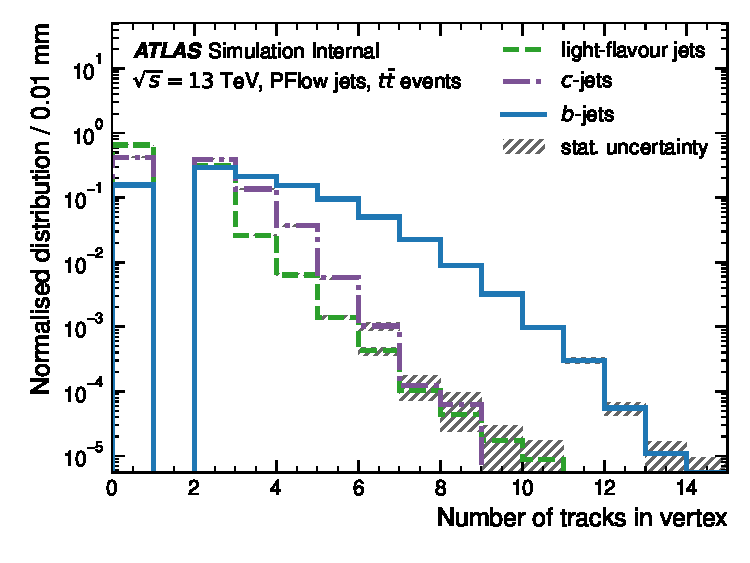
\includegraphics[width=0.32\linewidth]{\figpath/JetFitter_nTracksAtVtx_ttbar.pdf}
} 
\subfloat[]{ 
    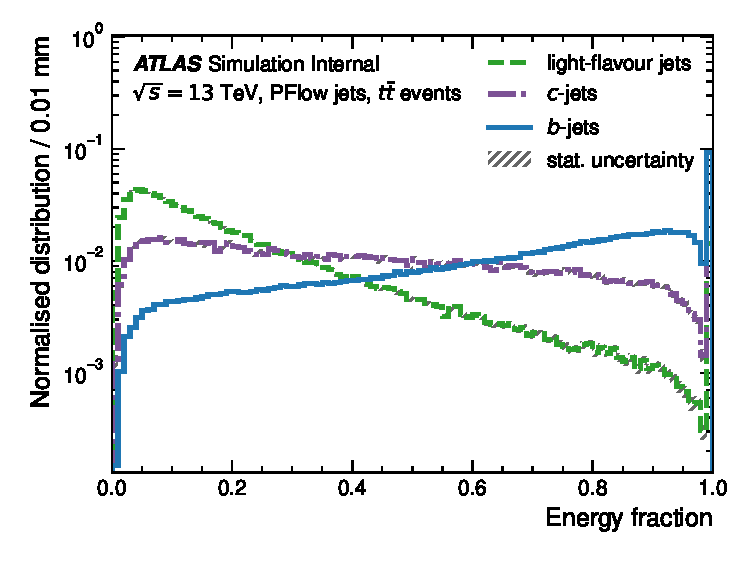
\includegraphics[width=0.32\linewidth]{\figpath/JetFitter_energyFraction_ttbar.pdf}
} 
     \subfloat[]{ 
    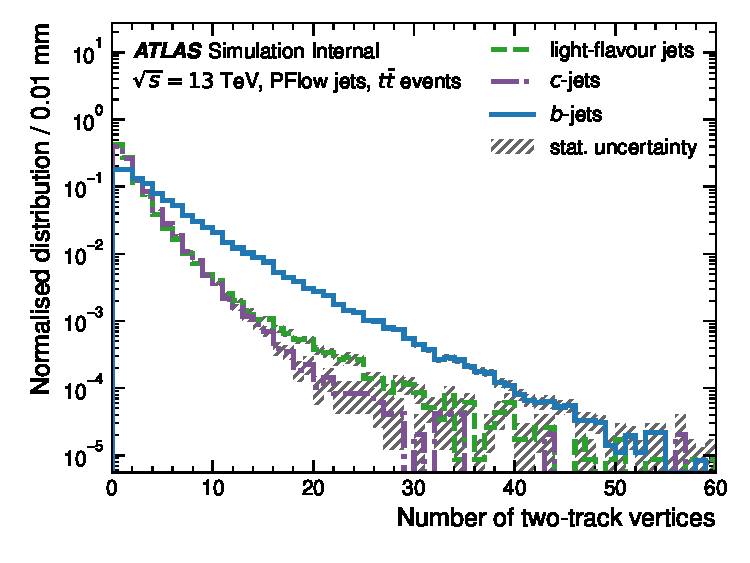
\includegraphics[width=0.32\linewidth]{\figpath/JetFitter_N2Tpair_ttbar.pdf}
} \\ 
\subfloat[]{ 
    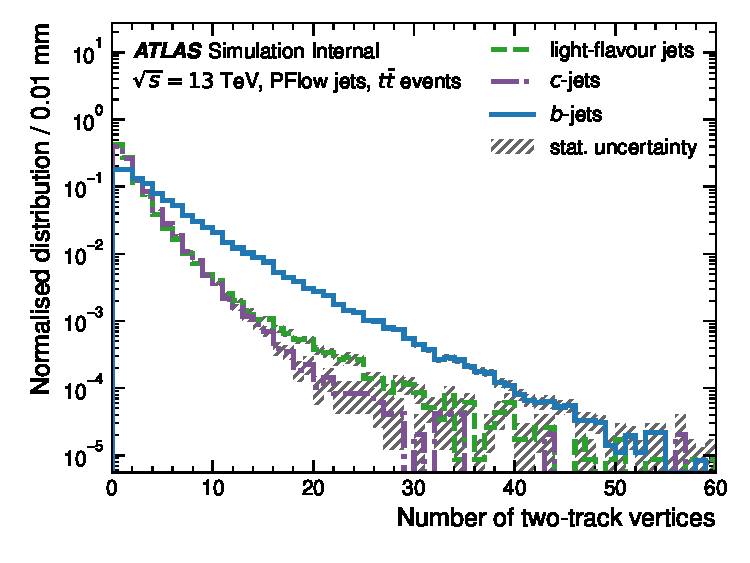
\includegraphics[width=0.32\linewidth]{\figpath/JetFitter_N2Tpair_ttbar.pdf}
} 
\subfloat[]{ 
    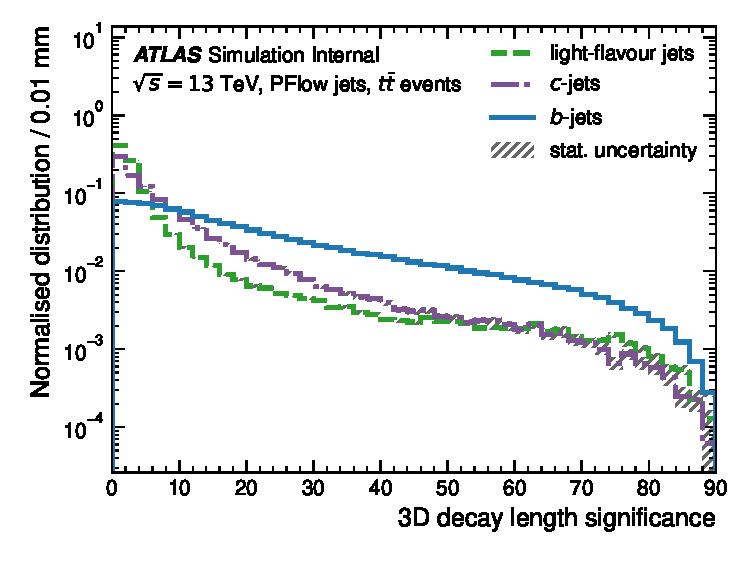
\includegraphics[width=0.32\linewidth]{\figpath/JetFitter_significance3d_ttbar.pdf}
} 
\subfloat[]{ 
    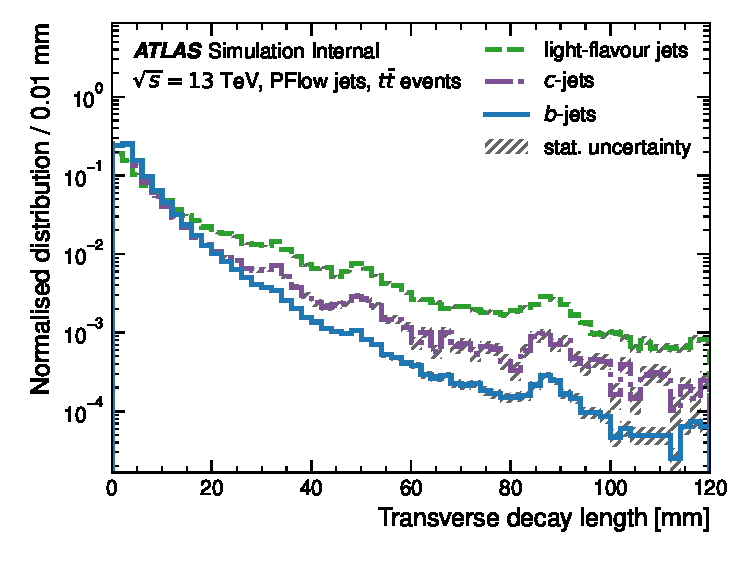
\includegraphics[width=0.32\linewidth]{\figpath/JetFitterSecondaryVertex_displacement2d_ttbar.pdf}
} 
\caption{An illustration of some of the JF inputs \cite{ANA-FTAG-2019-07}.}
\label{fig:jf-inputs}
\end{figure}


The second block of variables were included to optimize the sensitivity to \Pqc-tagging. For \Pqb-jets, we only expect one displaced vertex, so these variables are only calculated when JF finds \emph{exacly one} displaced vertex. These variables quantify the (2d and 3d) distance of the SV, its invariant mass, the energy of the trakcs and track muliplicity of the displaced vertex. 
Additionally, since the \Pqc-hadron has a lower decay multiplicity than the \Pqb-hadron decay, this means each of the \Pqc-hadron tracks carry a larger proportion of the energy and have a wider opening angle \cite{ATL-PHYS-PUB-2017-013}. 
The min, max, and avg $\eta$ of the tracks in the jet and the tracks in the displaced vertex and the tracks in the jet give us a handle on this discrimination variable.

\begin{table}[h!]
\centering
\begin{tabular}{p{3cm} | p{11cm}  } 
\textbf{Input} & \textbf{Description}  \\
\hline
\hline
	$m_{JF}$ & Invariant mass of the tracks attached to displaced vertices \\
	$f_E$ & Fraction of the energy in the displaced vertices compared to the jet's energy \\
	$\Delta R(\vec{p}_{jet}, \vec{p}_{vtx})$ & \\
	$S_{xyz}$ & Average significance of all of the displaced vertices \\
	$N_{trk}$ & Number of tracks associated to the fitted displaced vertices along the cascade decay chain \\
	$N_{2-\text{trk-vtx}}$ & Number of 2 track vertices (before the decay chain fit) \\
	$N_{1-\text{trk-vtx}}$ & Number of the single track vertices (after the decay chain fit) \\
	$N_{\geq 2-\text{trk-vtx}}$ & Number of the multi-prong displaced vertices (after the decay chain fit) \\
	\hline
	$L_{xyz}$(SV) & 3d distance from the first displaced vertex  \\
	$L_{xy}$(SV) &  transverse distance from the first displaced vertex \\
	$m_{trk}$(SV) & Mass of the tracks associated to the first displaced vertex \\
	$E_{trk}$(SV) & Energy of the tracks in the first displaced vertex \\
	$f_E$(SV) & Energy fraction of the tracks in the first displaced vertex compared to the energy of the jet \\ 
	$N_{\text{trk}}$(SV) & Number of tracks attached to the first displaced vertex \\
	$\eta_{\text{trk}}^{\text{max, min, avg}}$(SV) & The maximum, minimum, and average pseudorapidity of the tracks in the displaced vertex \\
	$\eta_{\text{trk}}^{\text{max, min, avg}}$ & The maximum, minimum, and average pseudorapidity of the tracks in the jet\\	
	% Are these abs etas or w/r.t. the jet axis?
\end{tabular}
\caption{Features from the JF reconstruction that are fed as input to the DL1r tagger. The first block of variables quantifies the global properties of the displaced vertices and decay topology. The second set of variables just looks at the properties of the first displaced vertex which capture the differences between \Pqb-jets and \Pqc-jets.}
\label{tab:jf-inputs}
\end{table}




%\subsection{SMT}

\begin{enumerate}
	\item BR
	\item BR
\end{enumerate}

\begin{figure}[htb]
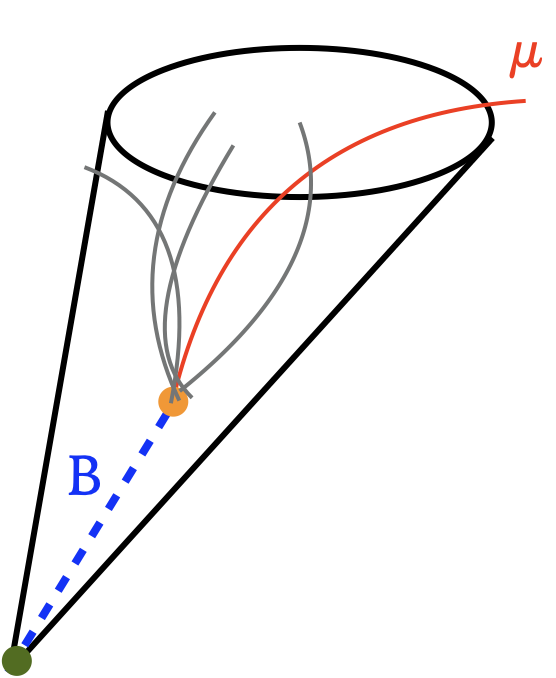
\includegraphics[width=.3\textwidth]{figures/ftag/SMT-image}
\caption{Illustration of a semileptonic $B$-decay}
\end{figure}

\begin{table}[h!]
  \centering
    \begin{tabular}{l | l } % <-- Alignments: 1st column left, 2nd middle and 3rd right, with vertical lines in between
      \textbf{Input} & \textbf{Description}  \\
      \hline
      \hline
  	$s_{d0}$ & $d_0 / \sigma_{d0}$: Transverse IP significance \\
	$s_{z0}$ & $z_0 \sin \theta / \sigma_{z0 \sin \theta}$: Longitudinal IP significance \\
%	$\log \pT^{frac}$ & $\log \pT^{track} / \pT^{jet}$: Logarithm of fraction of the jet $\pT$ carried by the track \\
%	$\log \Delta R$ & Logarithm of opening angle between the track and the jet axis \\    \end{tabular}
    \caption{Track features used as inputs for RNNIP and DIPS algorithms.}
    \label{table:inputs}
\end{table}

\textbf{I think Rafael added new variables too:}


